% (c) Jakub Stejskal
% Master Thesis
% Performance Testing and Analysis of Qpid-Dispatch Router
% Chapter 5
\chapter{Implementation}
\label{Implementation}
This chapter summarizes the implementation of components, which were described in the Chapter \ref{Analysis and Design}. The main part is the Agent module for MPT, which is implemented in Java and Groovy language. The second part is topology generator, which is python package for automatic generation of dispatch topology based on user's metadata. Since topology deployment is not part MPT or Topology generator, there is also described \emph{Ansible} and \emph{Docker} technology. Measurement data gathering and reporting is done by MPT parts which already been mentioned in the Chapter \ref{Analysis and Design}.   


\section{Used Technologies}
Messaging Performance Tool is a very large project with several parts. The most of MPT, such as command parsing, reporting, clients abstractions and so on, are written in Java language. But it is not pure Java code. For specify the test, which using MPT, is used Groovy language. Groovy is basically lightweight version of Java with several advantages. From my point of view are Groovy scripts more readable for those who are not more familiar with Java code. Groovy scrips are also used as reaction for specific commands for extension points, but this is deeply described in the Subsection \ref{MPT Preparations}.

On the other hand, Topology Generator is a new simple project. For easy integration to another projects, quick development and easy code preview I choose \emph{Python} language. Whole generator is created as one package, which is available for install on every machine with installed Python version 2.7 and higher. Already mentioned technologies are very common and almost every programmer have heard about Java and Python. In the following subsections I describe technologies, which are not common, but they are widely in use.

\subsection{Ansible}
Ansible \cite{Ansible} is simple automation framework which allow users to automate daily tasks on multiple nodes or containers. Basic types of tasks which can be automated by Ansible are:

\begin{itemize}
	\item \textbf{Provisioning}\,---\,setup the various servers user need in network infrastructure.
	\item \textbf{Configuration management}\,---\,change configuration of an application, operation system or device. Basically it allows start, stop and restart services, install or update application or perform a wide variety of other configuration tasks.
	\item \textbf{Application deployment}\,---\,automatic deployment of internally developed application to your systems with all dependencies.
\end{itemize}

Ansible scripts are written in YAML language which makes Ansible scripts to easy readable for humans and very simple to manage. Another advantage is that user does not even need to know commands used to accomplish a particular tasks. All is needed to specify what state does user wants the system to be in. Ansible is available on multiple systems with really short list of dependencies; Linux based systems needs Python and Windows need PowerShell, both systems needs SSH.

\begin{figure}[H]
  \centering
  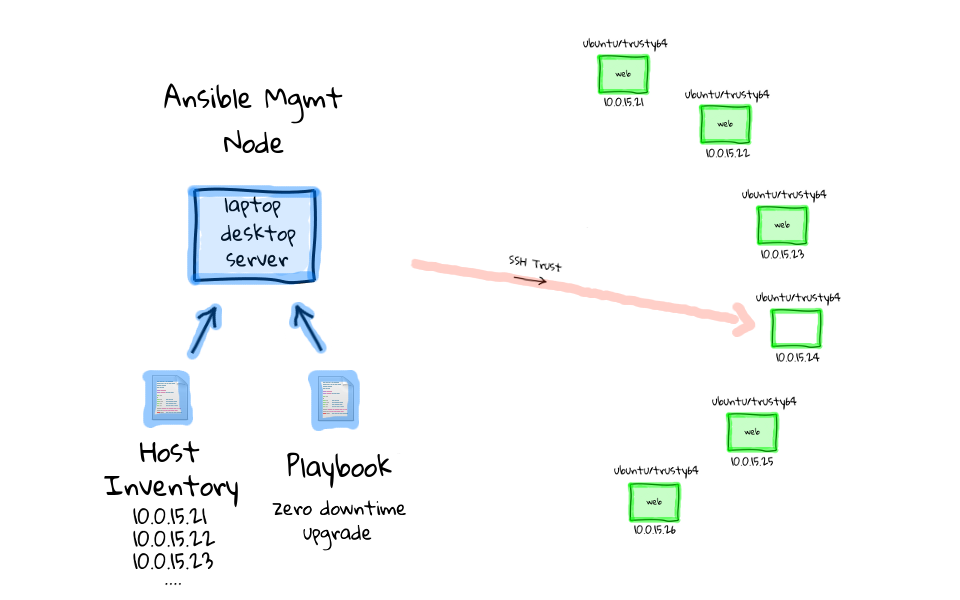
\includegraphics[width=10cm]{obrazky-figures/ansible.png}
  \caption{Ansible architecture. \todo{Placeholder}}
  \label{fig:ansible_architecture}
\end{figure}

In this thesis is Ansible used for several tasks; main is to deploy systems on specific nodes. As I want to run performance tests of Qpid-dispatch on multiple topology scenarios it is necessary to do system deployment quickly and automated which is easy with Ansible. System deployment contains MPT installation, Qpid-dispatch installation and other services based on testing scenario. The next task is to create and deploy configuration files for each router machine. This task runs Topology generator and based on its output create configuration file for each machine. 


\subsection{Docker}
Docker \cite{Docker} is an open platform which provide developing, shipping and running application separately from your infrastructure. Basically, docker is specific type of virtualization technology which allows the ability to package and run an application in a loosely isolated environment called a container. Docker containers are lightweight virtual machines run directly within the host machine's kernel. This means that you can run more containers than virtual machines on specific hardware, even you can run containers on virtual machines. 

Docker container are build up from a dockerfile where are specified container attributes such as OS in container, environment variables and steps for install applications. Output of build command is docker image. This image is ready for run as a container with another specific attributes such as exposes ports. Containers can be attach to same network which allow communication between all containers in the same network.

\begin{figure}[H]
  \centering
  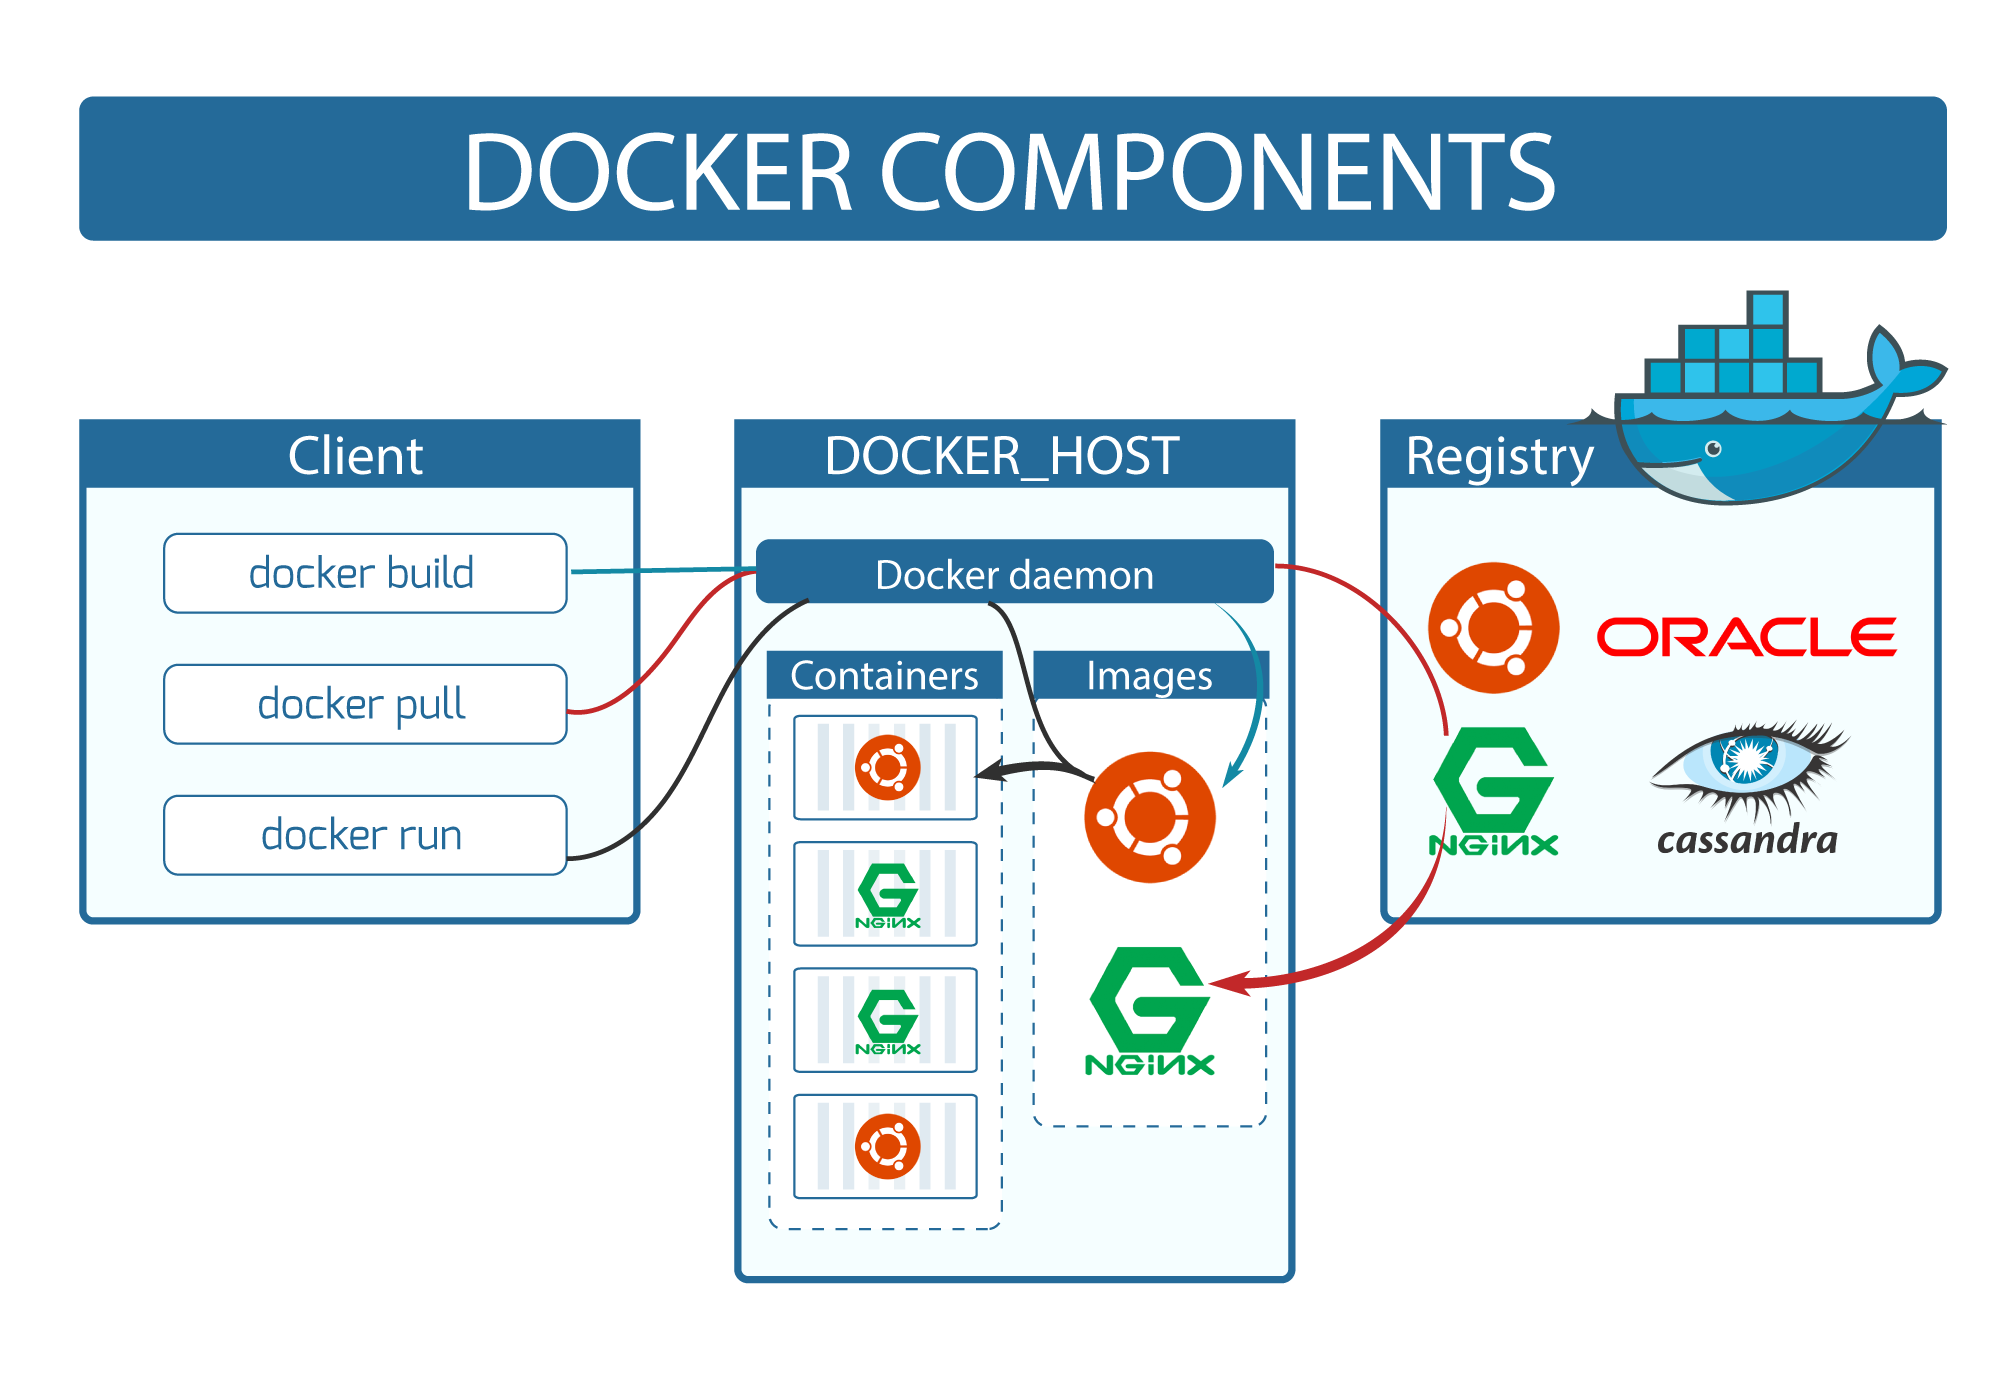
\includegraphics[width=10cm]{obrazky-figures/docker.png}
  \caption{Docker architecture. \todo{Placeholder}}
  \label{fig:ansible_architecture}
\end{figure}


Since docker is able to run services such as Qpid-dispatch very easily and also allow communication between containers, we are able to deploy MPT with proper SUT on containers and analyze behavior in the container network or just run MPT on single machine. However, for proper performance results we needs real machines, docker containers are uses only for testing and trying some basic stuffs with MPT.


\section{Topology Generator}

\subsection{Template Generator}

\subsection{Generation of Variables}

\subsection{Configuration Files Generation and Deployment}

\section{Qpid-Dispatch Performance Module}

\subsection{MPT Preparations}
\label{MPT Preparations}

\subsection{Agent Module Integration}

\subsection{Groovy As an Extension Handler} 

\subsection{Agent Capabilities}

